\section{Intervals of Understood Behavior} \label{res:understood}

	A cursory review of the orbit diagrams in Figure \ref{fig:orbits} reveals that the overall behavior of the systems seems to be quite similar, with many regions being nearly identical while some are entirely different. This section will focus on the former type of parameter intervals, briefly covering regions were the dynamics are fairly straightforward/similar to well known behaviors. In addition to the numerical bounds for each interval, we will include the special parameter names with orbit codings which will be introduced in the next section.

	Note that Figure \ref{fig:giters} provides graphical iteration of the positive critical point for most of the parameter values described below. These images may prove useful when trying to visualize how the system is changing at each parameter value.

	\underline{$c > .24604 \approx s_1^r$}

	For $c > .24604$, $f_c (x)$ behaves in a very similar manner to $Q_c (x)$ for $c > .25$ in that the plot is entirely above the reference line, as shown in Figure \ref{esc}. In both cases, all orbits escape because the function has no fixed points or periodic behavior so there is nothing to prevent all orbits from escaping to $\infty$ (hence the white space in our orbit diagrams). This interval of universal escape ends when the $f_c (x)$ undergoes a saddle node bifurcation at $c \approx .24604 \approx s_1^r$. This change is analogous to the saddle node of $Q_c (x)$ which occurs at $c = .25$. 

	\begin{figure}
		\centering
		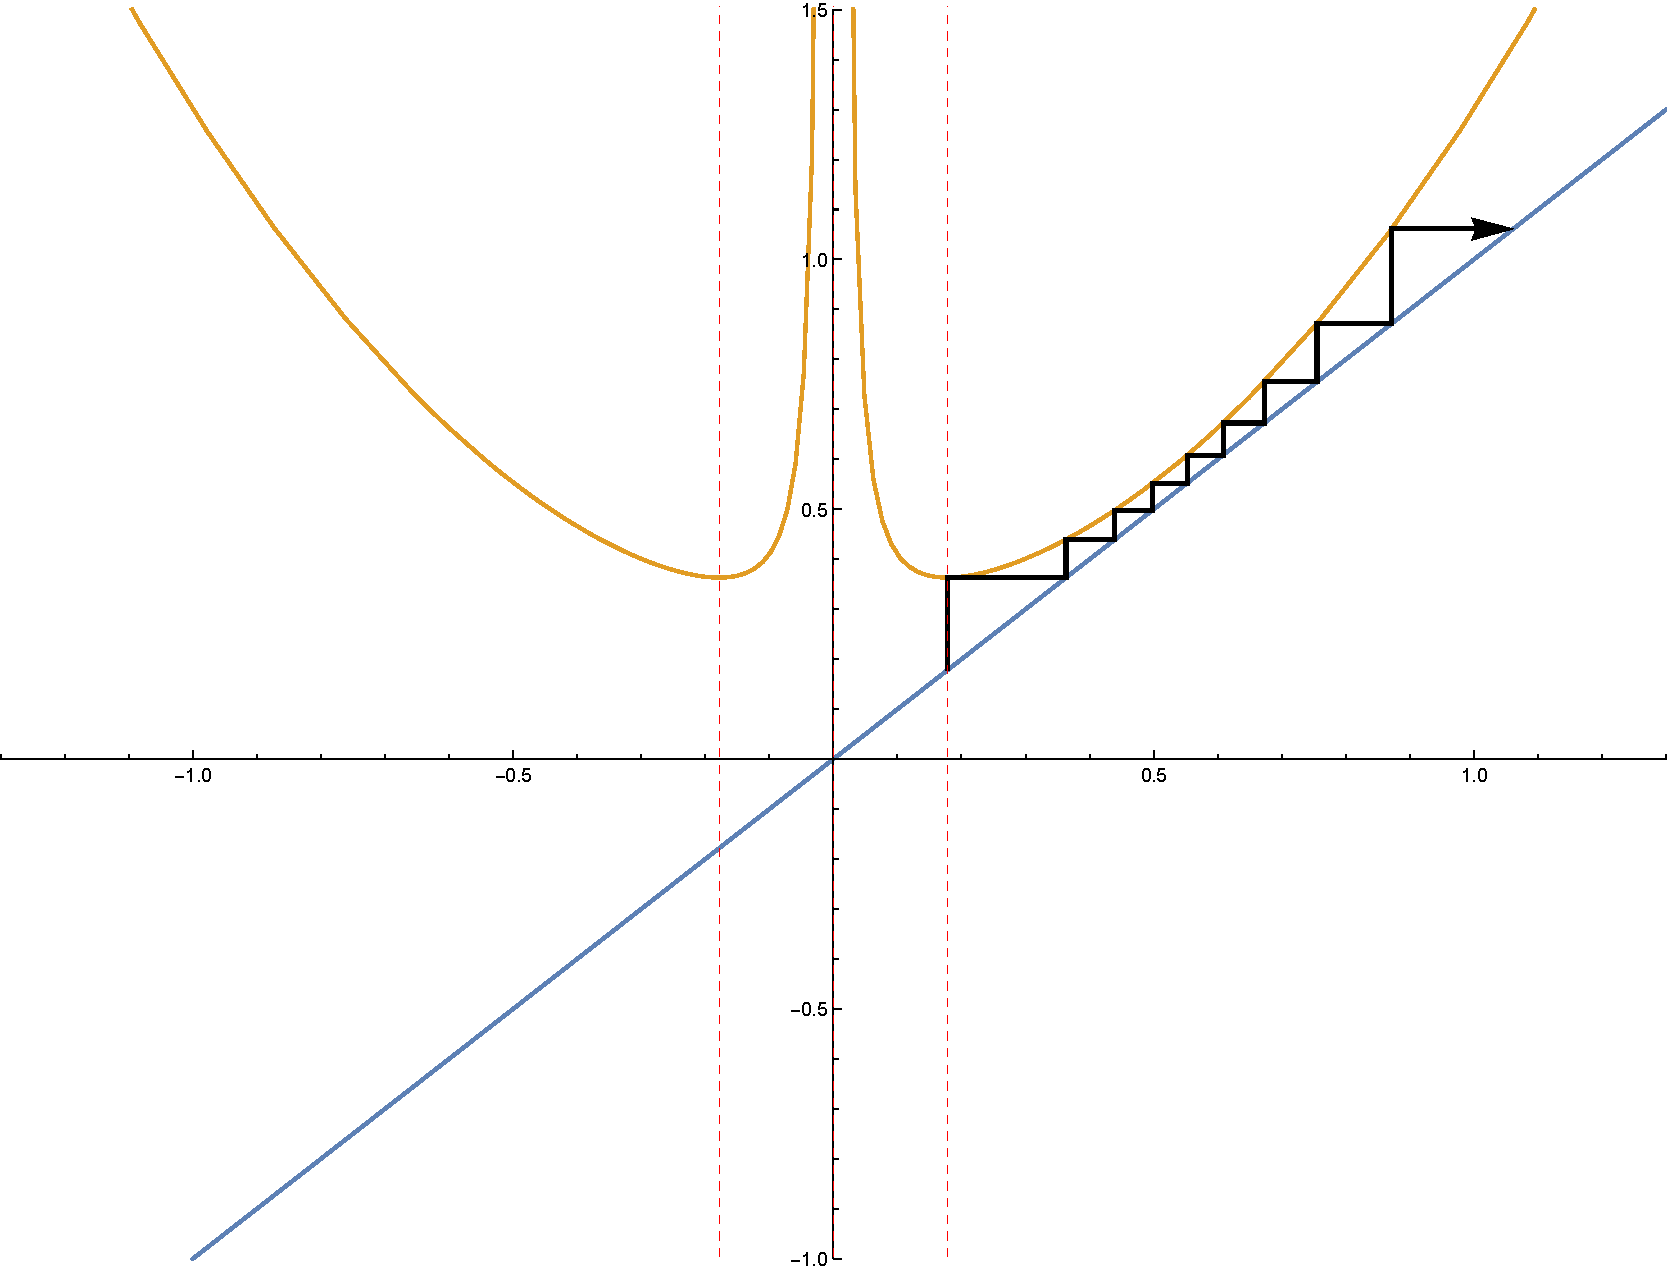
\includegraphics[width=.75\textwidth]{./img/plot03}
		\caption{Graphical iteration of the positive critical point under $x^2 + .3 + \frac{.001}{x^2}$, showing escape}
		\label{esc}
	\end{figure}

	

	\underline{$c \in (-.03255, .24604) \approx (h_2^{CLP_c}, s_1^r)$}

	Following the saddle node bifurcation and until $c \approx -.035$, the perturbed system seems to be going through the standard period doubling route to chaos that is similar to the behavior exhibited by $Q_c (x)$ for $c \in (-2,.25)$. Figure \ref{fig:perdub} shows a zoom of the perturbed map over $c\in (-.35, .05)$ along side the orbit diagram for $Q_c (x)$. While the exact shapes of the two images are slightly different, it is readily apparent that the two systems are exhibiting nearly identical behavior, that is to say that they appear to be topologically equivalent. For example, we can trace out the sequence of period doublings from 1 to 2 to 4 and so on, as well as match other windows (especially the period three which is very clear on both diagrams). The reason for this similarity is that on this parameter interval, the bimodal map $f_c (x)$ is actually acting as a unimodal map because the entire curve is above 0, meaning that all orbits are acting on only the right portion of the curve after at most one iterate. Additionally, this unimodal map has a very similar shape to that of the quadratic map, causing a similar sequence of bifurcations to occur. Thus this interval has been reduced to already known results and we expect that the methods from the study of the $Q_c (x)$ map would be able to describe the behavior observed over this parameter interval.

	\begin{figure}[h]
		\centering
		\begin{subfigure}[b]{0.48\textwidth}
				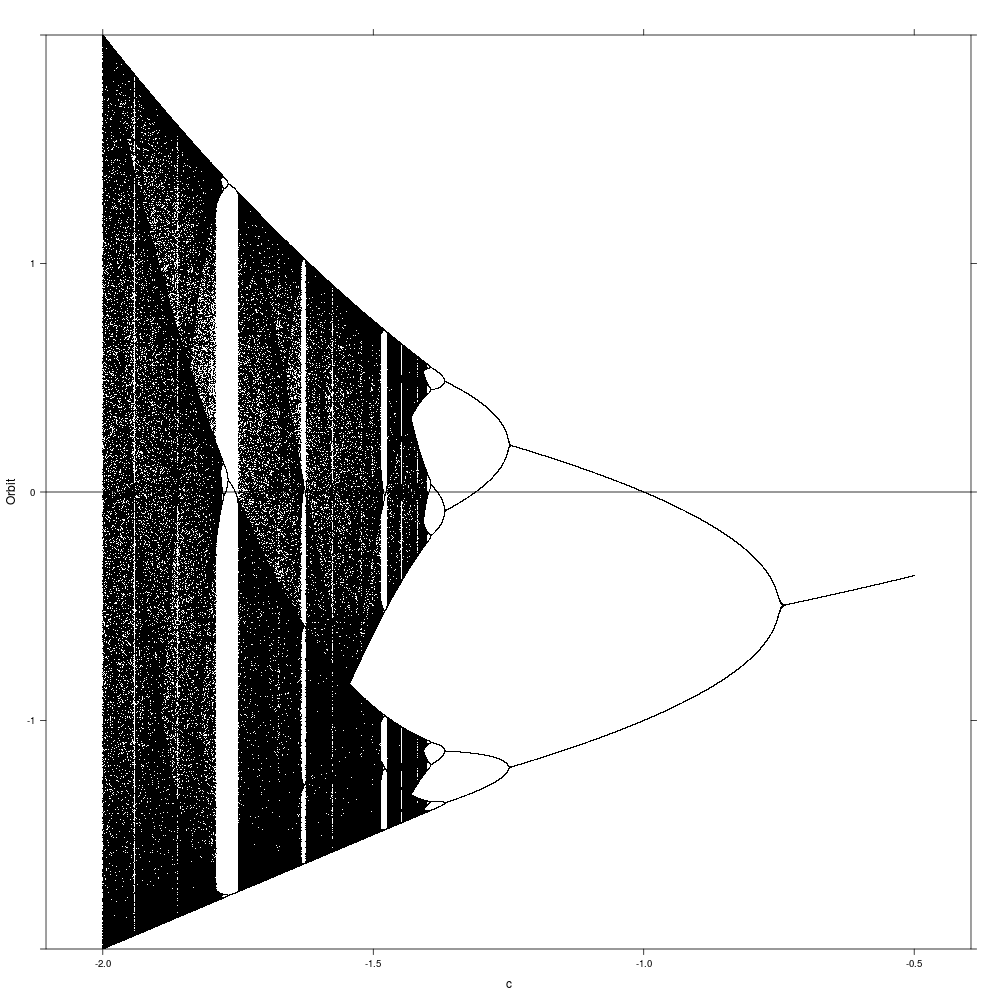
\includegraphics[width=\textwidth]{./img/stdperdub}
				\caption{Orbit Diagram for $Q_c (x)$ where $c\in (-2, -.5)$}
		\end{subfigure}
		\begin{subfigure}[b]{0.48\textwidth}
				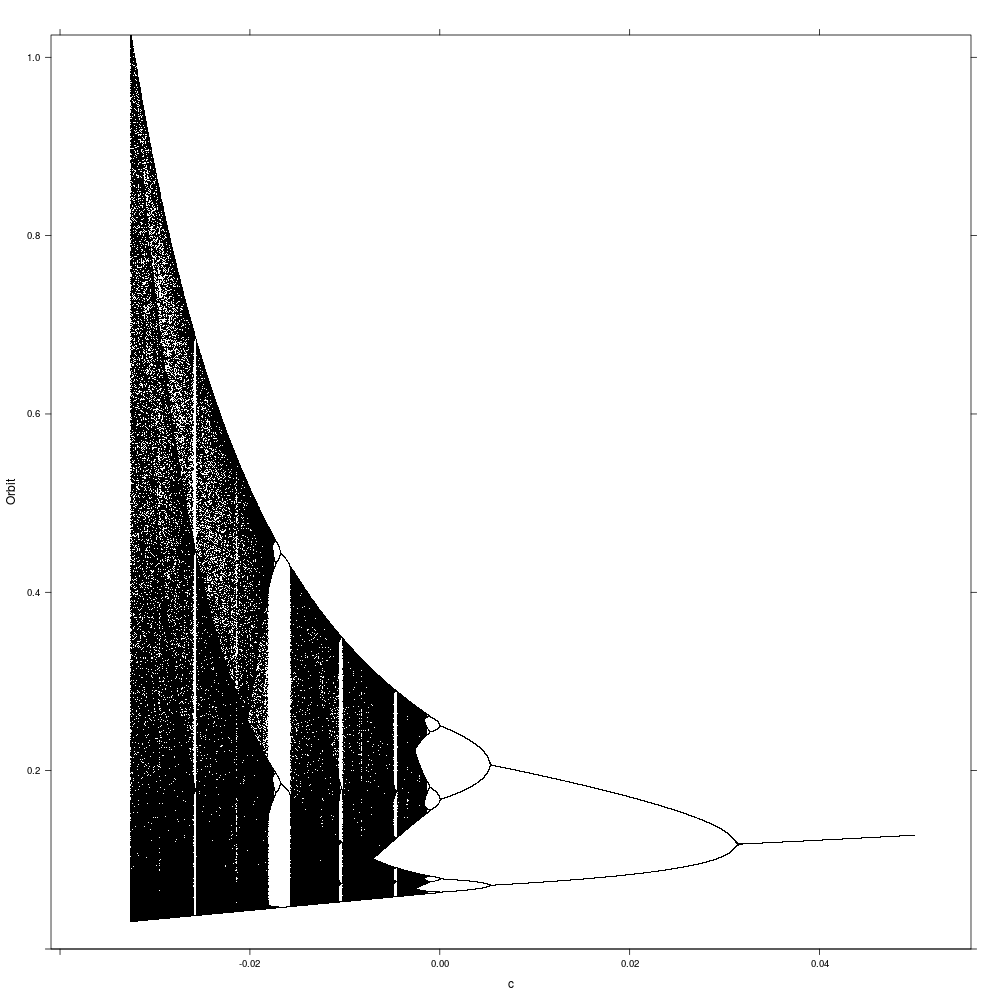
\includegraphics[width=\textwidth]{./img/pertperdub}
				\caption{Orbit Diagram for $f_c (x)$ where $c\in (-.035, .05)$}
		\end{subfigure}%
		\caption{Orbit diagrams of the original system and the perturbed system}\label{fig:perdub}
	\end{figure}

	\underline{$c\in (-.0632456, -.03255) \approx (z_1^{C0}, h_2^{CLP_c})$}

	For $c < -.03255$, the critical value first escapes by mapping just to the right of the right hand fixed point and then continuing to infinity. Thus the dynamics on this interval would be very similar to the dynamics of $Q_c (x)$ for $c < -2$ where the critical orbit escapes leaving a Cantor set of points which stay bounded. Again similar techniques from the quadratic map study would likely be able to prove that the dynamics on this remaining Cantor set would exhibit chaotic behavior when considered under a conjugacy with the Shift Map on two symbols. As $c$ continues to drop, this first iterate of the critical value is mapped higher and higher up the singularity around 0 until $c \approx -.0632456 \approx z_1^{C0}$ where $f_c (C) = 0$ as we see below:
	\[
		f_c (C) = 0 \Ra \left (\beta^{\frac{1}{4}}\right)^2 + c + \frac{\beta}{\left (\beta^{\frac{1}{4}}\right)^2} = 0 \Ra c = -2 \beta^{\frac{1}{2}} \Ra c = -2 (.001)^{\frac{1}{2}} \Ra c \approx -.0632456 \approx z_1^{C0}
	\]
	Thus at the parameter value $z_1^{C0}$ the $n^{th}$ iterate of the critical point maps directly to $\infty$ for $n > 1$.

	\underline{$c\in (-.092495, -.0632456) \approx (h_2^{CLP_c}, z_1^{C0})$}

	As $c$ decreases from $z_1^{C0}$, the second iterate of the critical point moves down the left side of the singularity until the parameter value $c \approx -.092495$ which is the point where the first iterate is small enough such that the second iterate is exactly the right hand fixed point $P_c$. Once the second iterate lands below $P_c$, the behavior is no longer similar to the behavior of $Q_c (x)$ for $c < -2$. Again refer to Figure \ref{fig:giters} for graphical iteration depicting most of the changes discussed here

	\underline{$c\in (-.241073, -.092495) \approx (p_1^{-C}, h_2^{CrP_c})$}

	This interval is the subject of the following sections where it will be described in detail.

	\underline{$c \in (-2.1, -.241073) \approx (h_2^{ClP_c},p_1^{-C})$}

	In this interval, $f_c$ again acts in a similar manner to the $Q_c (x)$ map because whenever the critical orbit stays far enough away from the singularity, the global geometry of the curve has more influence than the singularity. However we do note several significant deviations from the $Q_c (x)$ dynamics, most notably where the map ``should'' undergo a period doubling bifurcation. Instead, the $f_c (x)$ orbit diagram seems to be filling an interval of orbit values, indicating more complicated behavior. Additionally, the orbit diagram isn't nearly as well filled in at other points (even though the same number of iterates were plotted in either case). This is likely due to the many complicated ways by which points may escape through the ``trap door'' near $x=0$. Further study would be required to fully understand the behavior on this interval and appreciate its similarity/dissimilarity to $Q_c (x)$.

	\underline{$c < -2.1 \approx h_2^{ClP_c}$}

	On this interval, the critical orbit again escapes because its second iterate lands to the right of the right hand fixed point $P_c$. Again the dynamics on this interval would be similar to that of the $Q_c (x)$ map for $c < -2$ where there would be a Cantor set of points remaining. Here though, instead of two preimages of every escaping interval as we have with $Q_c (x)$, $f_c (x)$ would have four preimages of the escaping interval due to its bimodal shape. Thus instead of the middle thirds Cantor set for $Q_c (x)$, we would likely have a middle ``four ninths'' Cantor set of points which do not escape. The dynamics of the points in this set should be conjugate to the shift map on four symbols.